\chapter{Our Approach}\label{cap:our_approach}

\section{UQ Proposed Dataflow}
Summarizing, we proposed a workflow to quantify the uncertainty in large-scale spatio-temporal models, figure \ref{fig:workflow}. The workflow is divided into three main steps, the fitting process, the clustering and the queries. We illustrate the use of the workflow with  two queries, sections \ref{sub:gldMixtureWorkflow} and \ref{sub:InfomationEntropyRegionWorkflow}.

\begin{figure}[H]
    \centering
    \includegraphics[width=1\textwidth]{img/Diagram.png}
    \caption{Proposed workflow. The workflow was divided in three steps, (a) the fitting process, (b) the clustering of the GLDs and, (c) the queries over the results of the clustering process.}
    \label{fig:workflow}
\end{figure}

\subsection{Clustering}
In section \ref{gldShape} we discussed the different shapes of the GLD and define the regions of the $(\lambda_{3}, \lambda_{4})$ space where the shapes are similar. In Figure \ref{fig:similarityshapesGLD}, we show how  similar values of $\lambda_{3}$ and $\lambda_{4}$ lead to similar shapes. This fact suggests that one can clusterize the \textit{GLD} based on its lambda values. The  result of this clusterization are groups of \textit{GLDs} with similar shapes (behaviors).

In addition to $\lambda_{3}$ and $\lambda_{4}$, which  represent the right and left tails of the distribution, we have also to consider $\lambda_{2}$, as the latter represents the dispersion of the distribution. 

Then, in this step of our workflow, we clusterize the \textit{GLDs} using $\lambda_{2}$, $\lambda_{3}$ and $\lambda_{4}$ values. The final result of this step is:
\begin{equation}
S_{\mathcal{C}}(s_{i},t_{j},GLD_{k},clusterID)
\end{equation}
where:
$clusterID$ represents the ID of the cluster to which the \textit{GLD} at the spatio-temporal location $(s_{i},t_{j})$ belongs.

With the \textit{GLD} clusterized, we can use this result to characterize the uncertainty in a particular spatio-temporal region, or to measure numerically the corresponding uncertainty. In subsections \ref{sub:gldMixtureWorkflow} and \ref{sub:InfomationEntropyRegionWorkflow}, we describe how those approaches are implemented (see Figure \ref{fig:workflow}).

\section{Fitting a GLD to a spatio-temporal dataset}
In the more general case the computational model $\bm{q}=\mathcal{M}(\bm{\theta})$ represents the spatio-temporal evolution of a complex systems, and the \textit{QoI} $\bm{q}$ could be represented as:  

\begin{equation} \label{eq:spatio_temporal}
\mathbf{Q} = (\mathbf{q}(s_{1},t_{1}),\mathbf{q}(s_{2},t_{2}),...,\mathbf{q}(s_{n},t_{n}))  
\end{equation}
where:
\begin{itemize}
\item $(s_{1},t_{1}),(s_{2},t_{2}),....,(s_{n},t_{n}) \in \mathcal{S} \times \mathcal{T}\subseteq\mathbb{R}^{3}\times\mathbb{R}$ represent a set of distinct spatio-temporal locations, and
\item $\mathbf{q}(s_{i},t_{j})$ represents a value of the \textit{QoI} at the spatio-temporal location $(s_{i},t_{j})$
\end{itemize}
We could have many \textit{QoI}, but for simplicity here we are going to considere just one.

In the presence of a stochastic problem, on each spatio-temporal location $(s_{i},t_{j})$ we have many realizations of $q(s_{i},t_{j})$. A structure of a database to store this information can be modeled as:
\begin{equation}\label{eq:data_base_structure}
S(s_{i},t_{j},simId,q(s_{i},t_{j}))
\end{equation}
where $simId$ represents the \textit{id} of one simulation (realization).

The first step of our approach consists of trying to find the \textit{GLD} that best fits our simulations on each spatio-temporal location. The algorithms are described in the next section.

Given a random sample $q_{1}, q_{2}, q_{3},...,q_{n}$, the basic problem in fitting a statistical distribution to these data is that of approximating the distribution from which the sample was obtained. In our approach we divide this step in three task:
\begin{itemize}
\item Fit the \textit{GLD} to the data.
\item Evaluate the validity of the resulting \textit{GLD} on each spatio-temporal location.
\item Perform a ks-test to evaluate the quality of the fit on each spatio-temporal location.
\end{itemize}

The fitting process has been implemented following the algorithm \ref{alg:fitGLD}. Before starting the fitting process, we need to group all the simulations that correspond to the same spatio-temporal location $(s_{i},t_{j})$.  As a result we get a new dataset $S^*(s_{i},t_{j},<q_1,q_2,..,q_n>)$, where $q_i, 1 \le i \le n$, represents a vector of all the values of $q$ at point $(s_{i},t_{j})$.

\subsection{Fitting process}
\label{gldFitProcess}
Now, for each spatio-temporal location $(s_{i},t_{j}) \in \mathcal{S} \times \mathcal{T}$ we use a function of the GLDEX R package described in section \ref{GLDEX}, to fit the \textit{GLD} to a vector $<q_1,q_2,..,q_n>$, line 2 of algorithm \ref{alg:fitGLD}. As a result of this task we get the lambda values of the \textit{GLD} that best fit the dataset at each spatio-temporal location, equation \ref{eq:S_GLD}.
\begin{equation}\label{eq:S_GLD}
S'(s_{i},t_{j},GLD(\lambda_{1}, \lambda_{2}, \lambda_{3}, \lambda_{4}))
\end{equation}

\subsection{GLD validity check}
As we mention in section \ref{GLD} the \textit{GLD} is not always valid, it depends of the $\lambda_{3}$  and $\lambda_{4}$ values. The evaluation of the validity of the \textit{GLD} is straightforward, if $\lambda_{3}$  and $\lambda_{4}$ are in the gray regions of Figure \ref{fig:validGLD} the \textit{GLD} is not valid, on the other case is valid.

The validity check is performed in line 3 of the algorithm \ref{alg:fitGLD}, and as a result we get:
\begin{equation}
S_{validity}(s_{i},t_{j},valid(s_{i},t_{j})),
\end{equation}
where:
\begin{equation}
  valid(s_{i},t_{j}) =
  \begin{cases}
    1 & \text{if GLD is valid in $(s_{i},t_{j})$} \\
    0 & \text{otherwise}
  \end{cases}
\end{equation}

\subsection{Quality of the fit}
\label{Quality of the fit}
Now at the remaining points, where the \textit{GLD} is valid, we need to evaluate how good is the fit. That is, we evaluate whether the \textit{GLD} (PDF) correctly describes the dataset. We use here the Kolmogorov-Smirnov test (KS-test). The KS-test  determines if two datasets differ significantly. In this case, these datasets are: the original dataset and a second one generated using the fitted GLD. As a result, this test returns two values: a Kolmogorov-Smirnoff Distance (D); and a p-value, line 5 of algorithm \ref{alg:fitGLD}. The distance D is the maximum distance between both cumulative density functions (CDF), as shown in Figure \ref{fig:D_distance}. A small distance means that both, the dataset and the fitted PDF, are similar. 

\begin{figure}[ht]
    \centering
    \includegraphics[width=0.45\textwidth]{img/D_distance.png}
    \caption{Illustration of the two-sample Kolmogorov–Smirnov statistic. Red and blue lines each correspond to an empirical distribution function, and the black arrow is the two-sample KS statistic.}
    \label{fig:D_distance}
\end{figure}

The second value, the p-value, is a more robust test, as it helps us to determine the significance of our results. Suppose we have two hypotheses, the null hypothesis  is that our PDF is a good fit to our dataset, and the alternative hypothesis  is that it is not. Then, a small p-value (typically $\leq 0.05)$ indicates strong evidence against the null hypothesis, so you reject the null hypothesis. A large p-value $(> 0.05)$ indicates weak evidence against the null hypothesis, so you fail to reject the null hypothesis. p-values very close to the cutoff (0.05) are considered to be marginal (could go either way). 

At the end of this task we have two new multidimensional arrays with the values of $\mathcal{D}$ and \textit{p}-value on each spatio-temporal locations.
\begin{equation}
S_{\mathcal{D}}(s_{i},t_{j},\mathcal{D}(s_{i},t_{j}))
\end{equation}
\begin{equation}
S_{p_{value}}(s_{i},t_{j},p_{value}(s_{i},t_{j}))
\end{equation}

Finally, in line 7 of the algorithm \ref{alg:fitGLD} we store the lambda values of those \textit{GLDs} that are valid and return p-values greater than 0.05.

\begin{algorithm} 
\caption{Fitting the GLD to a spatio-temporal dataset}\label{alg:fitGLD}
\begin{algorithmic}[1] 
\Function{gldFit}{$S(s_{i},t_{j},<q_1,q_2,...,q_n>)$} 
\State $<\lambda_{1},\lambda_{2},\lambda_{3},\lambda_{4}> \gets \Call {fit.gld.lm}{<q_1,q_2,...,q_n>}$

\State $isValid_{(s_{i},t_{j})} \gets \Call {validityCheck}{<\lambda_{3},\lambda_{4}>}$
\If{$isValid_{(s_{i},t_{j})}$}
\State $[pvalue,D]_{(s_{i},t_{j})} \gets \Call{ks}{<\lambda_{1},\lambda_{2},\lambda_{3},\lambda_{4}>_{(s_{i},t_{j})}}$
\EndIf
\If{$pvalue_{(s_{i},t_{j})} > 0.05$}
\State $\Call{storeLambdas}{<\lambda_{1},\lambda_{2},\lambda_{3},\lambda_{4}>,s_{i},t_{j}}$
\EndIf
\EndFunction 
\end{algorithmic} 
\end{algorithm} 

%\section{Clustering Uncertain Data Based on GLD Similarity}
%\label{sec:clustering_gld}
%In chapter \ref{cap:gld} we exposed the two most important parametrizations of the \textit{GLD} and select the \textit{FMKL} as  the one to use for the rest of the  thesis. In this parameterization $\lambda_{1}$ represent the location of the \textit{GLD} and is directly related to the mean of the distribution. $\lambda_{2}$ is the scale, directly related to the standard deviation; and $\lambda_{3}$ and $\lambda_{4}$ represent the left and right tails of the distribution. Combinations of $\lambda_{3}$ and $\lambda_{4}$ can be used to estimate the skewness and kurtosis of the distribution.
%
%The uncertainty can be characterized in many different ways as we mention in chapter \ref{cap:backgroud}, but from the \textit{GLD} point of view, $\lambda_{2}$, $\lambda_{3}$ and $\lambda_{4}$ are the responsables of this. So, in this chapter we try to answer the research question 1, we formulate in the introduction:
%
%\begin{tcolorbox}
%\textbf{RQ1.} how to group the output of the UQ process based on the similarity of the uncertainty?
%\end{tcolorbox}
%
%First of all, in section \ref{sec:related_works} a brief review of some related works is performed. In this section, some advantage and drawbacks are highlighted, and some considerations about the possibilities of the use of the \textit{GLD} to solve some of the drawbacks are commented. Next, in section \ref{sec:clustering_gld} our hypothesis about the use of the \textit{GLD} to clusterized uncertain data, is presented. Sections \ref{sec:synthetic_I} and \ref{sec:synthetic_II} present two synthetics datasets and the results of the clustering technique. Those results help us to validate our hypothesis. Finally, section \ref{sec:conclusions} summarize and discuss the main results of the chapter.
%
%\subsection{Related Works}\label{sec:related_works}
%
%\cite{Jiang2011}
%
%\subsection{Clustering Based on GLD}\label{sec:clustering_gld}
%
%Our hypothesis is that, as the \textit{GLD} shape is characterized by $\lambda_{2}$, $\lambda_{3}$ and $\lambda_{4}$, and this shape change slowly with the change in the $\lambda_{i}$  values, we can group the uncertainty using clustering algorithms above $\lambda_{2}$, $\lambda_{3}$ and $\lambda_{4}$.  
%
%To test our hypothesis, we generate two synthetic datasets using 4 different probabiltiy density functions: Gaussian, Exponential, Uniform and Gamma. The structure of the datasets is represented in \ref{eq:multi_array}.  
%
%\begin{equation}\label{eq:multi_array}
%S(x_{i}, <v_{j}>) i=1.....n,j=1.....m
%\end{equation}
%
%where:
%\begin{itemize}
%\item n represent the number of objects of the dataset and,
%\item m represent the size of each object.
%\end{itemize}
%
%For example, the first object could be a Gaussian distribution with size = 1000, mean = 0 and standard deviation = 2, figure \ref{fig:normal_sample}. The datasets are described in details in sections \ref{sec:synthetic_I} and \ref{sec:synthetic_II}. 
%
%%Independently of the dataset, the first step is to fit the \textit{GLD} to each distribution. In the next subsection we present the algorithm used to do this.
%
%\subsubsection{Fit the GLD to a dataset}\label{sub:fitting_gld}
%When we generate a synthetic dataset, the next step is to find the \textit{GLD} that best fit $<v_{j}>$ on each $x_{i}$. As the fitting process is computationally intensive we implement a parallel algorithm using \textbf{R}. The seudo-code is shown in algorithm \ref{alg:fitGLDSyntheticDataset}.
%
%\begin{algorithm} 
%\caption{Fitting the GLD to a synthetic dataset}\label{alg:fitGLDSyntheticDataset}
%\begin{algorithmic}[1] 
%\Function{gldFit}{$S(x_{i},<v_1,v_2,...,v_{n}>)$} 
%\State $<\lambda_{1},\lambda_{2},\lambda_{3},\lambda_{4}> \gets \Call {fit.gld.lm}{<v_1,v_2,...,v_{n}>}$
%
%\State $isValid_{(x_{i})} \gets \Call {validityCheck}{<\lambda_{3},\lambda_{4}>}$
%\If{$isValid_{(x_{i})}$}
%\State $[pvalue,D]_{(x_{i})} \gets \Call{ks}{<\lambda_{1},\lambda_{2},\lambda_{3},\lambda_{4}>_{(x_{i})}}$
%\EndIf
%\If{$pvalue_{(x_{i})} > 0.05$}
%\State $\Call{storeLambdas}{<\lambda_{1},\lambda_{2},\lambda_{3},\lambda_{4}>,x_{i}}$
%\EndIf
%\EndFunction 
%\end{algorithmic} 
%\end{algorithm} 
%
%The algorithm receive a dataset represented by \ref{eq:multi_array} and, for each position $x_{i}$, call a function \textbf{\textit{fit.gld.lm}} from the \textbf{R} package \textbf{GLDEX} presented in section \ref{sec:gldex}, line 2 of the algorithm \ref{alg:fitGLDSyntheticDataset}. In line 3 we check the validity of the \textit{GLD} returned by the function (remember from chapter \ref{cap:gld} that the \textit{GLD} is not always valid). In line 5 a good-of-fit test is perform to be sure that each \textit{GLD} is a good representation for the dataset in $x_{i}$. Finally all the \textit{GLD} with $pvalue > 0.05$ are stored to be used in the next section.
%
%The final result of this process is a new dataset with the form:
%
%\begin{equation}\label{eq:multi_array2}
%S(x_{i}, <\lambda_{1},\lambda_{2},\lambda_{3},\lambda_{4}>)  i=1.....n
%\end{equation}
%
%\subsubsection{Clustering the GLD}\label{sub:clustering_gld}
%
%The clustering algorithm is trivial because the idea we try to test is that we can clusterize the uncertain data, using a simple k-means with a Euclidean distance over the $\lambda_{i}$ space.
%
%The dataset \ref{eq:multi_array2} is modified to remove $\lambda_{1}$. Then, a k-means algorithm is used first over $<\lambda_{2},\lambda_{3},\lambda_{4}>$ and second over $<\lambda_{3},\lambda_{4}>$. The results are discused in sections \ref{sec:synthetic_I} and \ref{sec:synthetic_II}.
%
%\subsection{Synthetic Data I}\label{sec:synthetic_I}
%To generate the first synthetic data set we use 11 probability density functions, where 5 are Gaussian, 5 Exponential, and one Uniform, figures \ref{fig:5_gaussian}, \ref{fig:5_exp} and \ref{fig:uniform}. The standard deviation of the 5 Gaussian distributions is $0.05*i$, with $i=1, 2, 3, 4, 5$, and we generate 90 samples of each distribution. This is, the first 90 objects where generated from a Gaussian distribution with standard deviation 0.05, and so on. Similarly, the rate of the 5 Exponential distributions is $i$, with $i=1, 2, 3, 4, 5$, and again we generate 90 samples of each one. Finally, 100 samples of a Uniform distribution between $[0, 1]$ were generated. In resume, we have 1000 objects, where the first 450 were sampled from a Gaussian distributions, the next 450 from an Exponential and the last 100 from a Uniform distribution. As we generate a synthetic dataset in this way, we have the ground truth of the clustering in the dataset. This ground truth is used to evaluate the clustering quality of our algorithms.
%
%\begin{figure}[H]
%    \centering
%    \includegraphics[width=0.8\textwidth]{img/gld_clustering/extra_images/5_gaussian.png}
%    \caption{Gaussian (Normal) distributions used to generate the synthetic dataset.}
%    \label{fig:5_gaussian}
%\end{figure}
%
%\begin{figure}[H]
%    \centering
%    \includegraphics[width=0.8\textwidth]{img/gld_clustering/extra_images/5_exp.png}
%    \caption{Exponential distributions used to generate the synthetic dataset.}
%    \label{fig:5_exp}
%\end{figure}
%
%\begin{figure}[H]
%    \centering
%    \includegraphics[width=0.8\textwidth]{img/gld_clustering/extra_images/uniform.png}
%    \caption{Uniform distribution used to generate the synthetic dataset.}
%    \label{fig:uniform}
%\end{figure}
%
%This dataset could be represented as a multidimensional array where for each position $x_{i}$, we have 1000 values $v_{j}$, equation \ref{eq:multi_array_datasetI}. In this case $i$ and $j$ vary from 1 to 1000 casually.
%
%\begin{equation}\label{eq:multi_array_datasetI}
%S(x_{i}, <v_{j}>) i,j=1, 2.....1000
%\end{equation}
%
%The fitting algorithm proposed in subsection \ref{sub:fitting_gld} is applied over \ref{eq:multi_array_datasetI}. The good-of-fit test return that all the \textit{GLDs} are good fit for its corresponding distribution. As a result the dataset \ref{eq:multi_array3} is genarated. 
%
%\begin{equation}\label{eq:multi_array3}
%S(x_{i}, <\lambda_{1},\lambda_{2},\lambda_{3},\lambda_{4}>)  i=1.....1000
%\end{equation}
%
%\subsubsection{Clustering using $\lambda_{2}$, $\lambda_{3}$ and $\lambda_{4}$}\label{syntheticI_l234}
%
%As we mention above, our idea is to test what happen if we use a simple k-means with euclidean distance over the $\lambda_{2}$, $\lambda_{3}$ and $\lambda_{4}$ values of the \textit{GLDs}. Similar to the paper \cite{Jiang2011}, as we use 11 \textit{PDFs} to generate the synthetic dataset I, we expect that the k-mean algorithm will return 11 clusters as well (one for each distribution). Then 11 is the number we use with the k-means algorithm.
%
%In figure \ref{fig:dataset1_l2l3l4} and table \ref{tab:dataset1_l2l3l4} the distribution of the clusters returned by the k-means is shown.
%
%\begin{figure}[H]
%    \centering
%    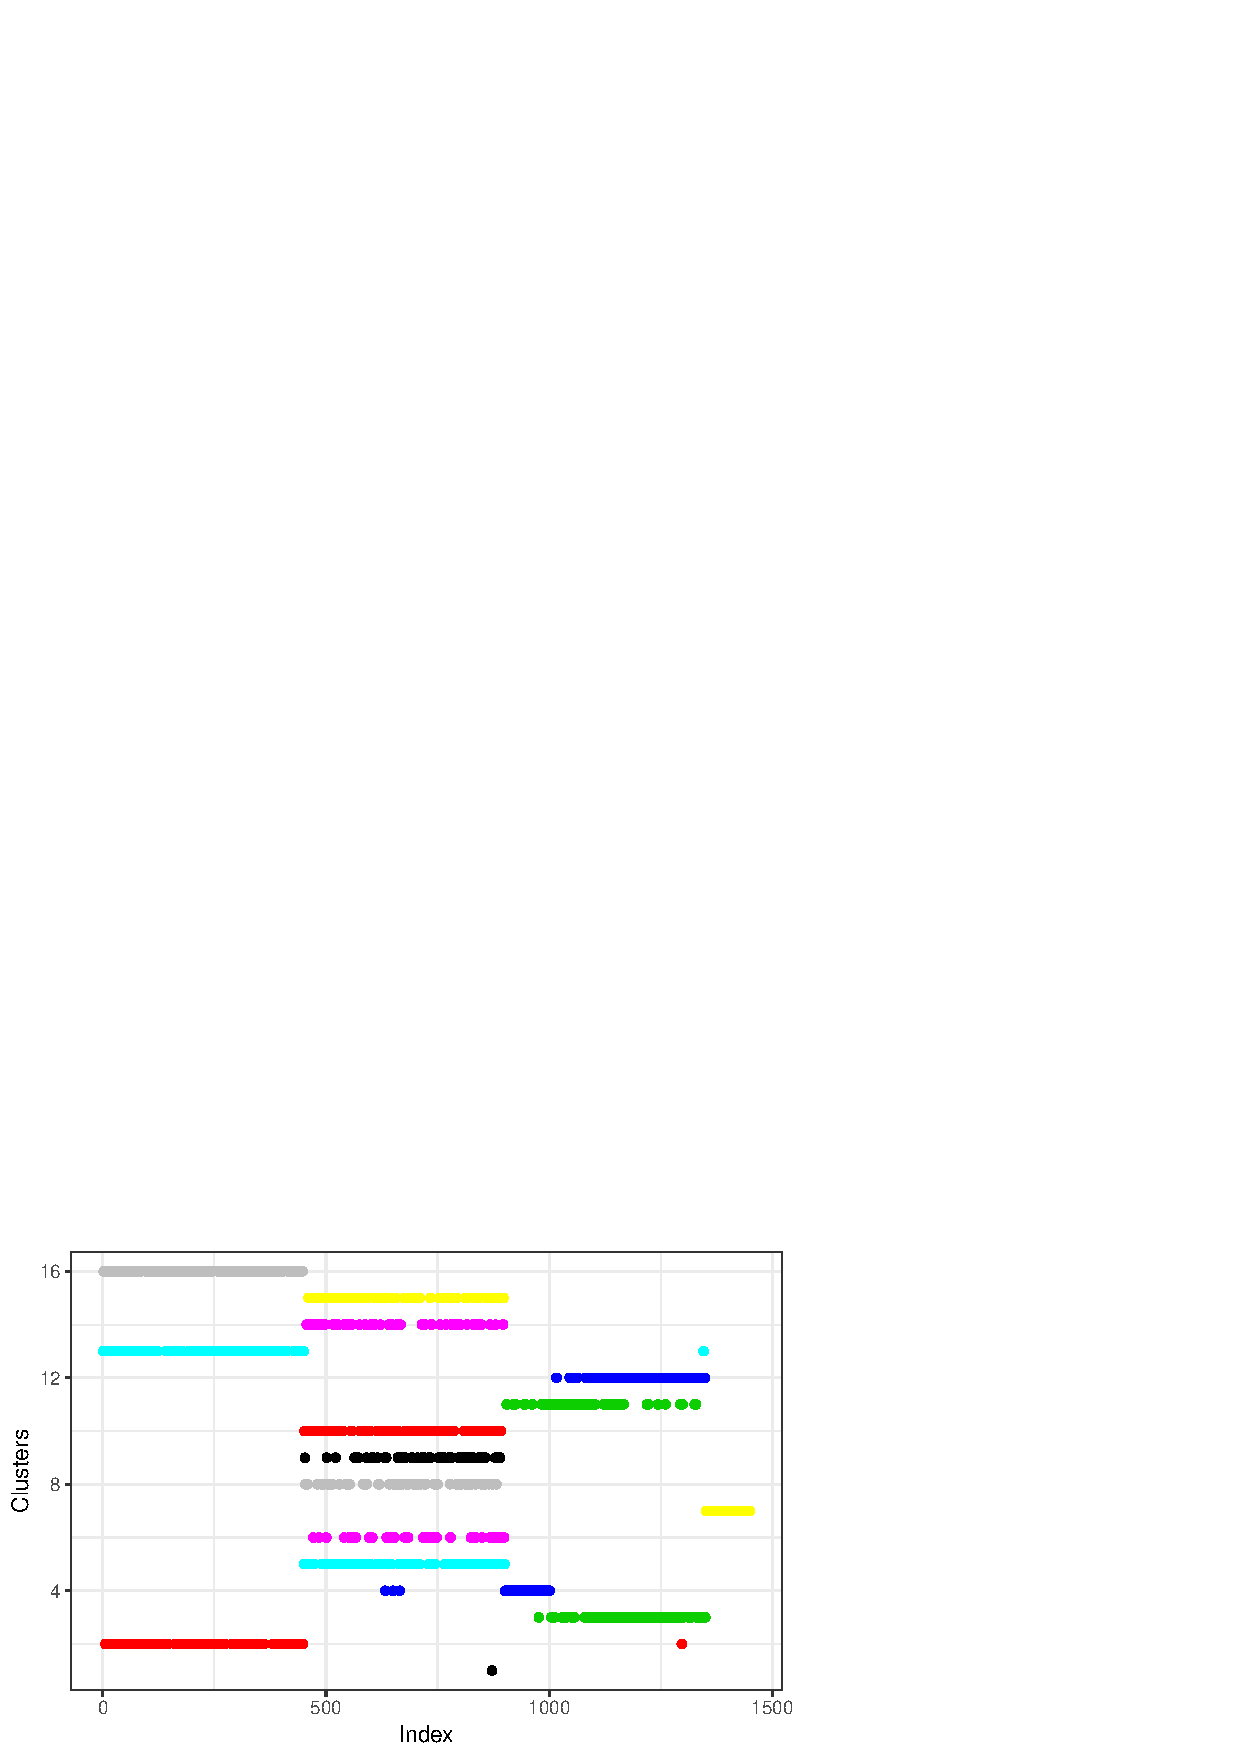
\includegraphics[width=0.8\textwidth]{img/gld_clustering/Dataset1/l2_l3_l4/intento_3/normal_exponential_uniform3.png}
%    \caption{Distribution of the clusters using k-means over the $\lambda_{2}$, $\lambda_{3}$ and $\lambda_{4}$ values of the \textit{GLDs}.}
%    \label{fig:dataset1_l2l3l4}
%\end{figure}
%
%\begin{table}[]
%\centering
%\caption{Distribution of the clusters using k-means over the $\lambda_{2}$, $\lambda_{3}$ and $\lambda_{4}$ values of the \textit{GLDs}.}
%\label{tab:dataset1_l2l3l4}
%\begin{tabular}{|c|c|c|}
%\hline
%Cluster & Type of Distribution & No. of Elements \\ \hline
%1       & Exponential          & 82              \\ \hline
%2       & Normal          & 93              \\ \hline
%3       & Exponential          & 5             \\ \hline
%4       & Normal               & 198              \\ \hline
%5       & Uniform               & 102              \\ \hline
%6       & Exponential               & 83             \\ \hline
%7       & Exponential              & 91             \\ \hline
%8       & Exponential          & 82              \\ \hline
%9       & Normal          & 90               \\ \hline
%10      & Exponential               & 84              \\ \hline
%11      & Normal          & 90              \\ \hline
%\end{tabular}
%\end{table}
%
%Remembered, the first 450 elements are normal distributions, the next 450 are exponential and the last 100 are uniform. Looking to those regions in general, the first observation is that we have 23 false positives, three in cluster 2, 18 in cluster 4 and two in cluster 5. The second observation is that, the normal distributions were grouped in 4 clusters (2, 4, 9 and 11), cluster 2 group perfectly it 90 elements with 2 false positives, clusters 9 and 11 group exactly its 90 elements each. The cluster 4 group the last 180 elements of the Normal distribution, with 18 false positives
%
%The Uniform distribution was grouped totally in cluster 5, with two false positives as was mention above. The last observation is that the algorithm can't separate the 5 Exponential distributions, but this is not a bad result as we will show soon. 
%
%In figures between \ref{fig:dataset1_l2l3l4_cl1} and \ref{fig:dataset1_l2l3l4_cl11} we show the \textit{PDFs} of all the distributions that belongs to the same cluster. If we take a look at figures \ref{fig:dataset1_l2l3l4_cl1}, \ref{fig:dataset1_l2l3l4_cl2}, \ref{fig:dataset1_l2l3l4_cl3}, \ref{fig:dataset1_l2l3l4_cl9}, \ref{fig:dataset1_l2l3l4_cl10} and \ref{fig:dataset1_l2l3l4_cl11} we see that the exponential distribution was well grouped. Really the problem is that the rate value of $0.05*i$ used to generate the exponential distribution does not have such a big difference between one and another.  
%
%\begin{figure}[H]
%    \centering
%    \includegraphics[width=0.8\textwidth]{img/gld_clustering/Dataset1/l2_l3_l4/intento_3/cluster1.png}
%    \caption{Cluster 1 returned by the k-means over the $\lambda_{2}$, $\lambda_{3}$ and $\lambda_{4}$ values of the \textit{GLDs}, synthetic dataset I.}
%    \label{fig:dataset1_l2l3l4_cl1}
%\end{figure}
%
%\begin{figure}[H]
%    \centering
%    \includegraphics[width=0.8\textwidth]{img/gld_clustering/Dataset1/l2_l3_l4/cluster4.png}
%    \caption{Cluster 2 returned by the k-means over the $\lambda_{2}$, $\lambda_{3}$ and $\lambda_{4}$ values of the \textit{GLDs}, synthetic dataset I.}
%    \label{fig:dataset1_l2l3l4_cl2}
%\end{figure}
%
%\begin{figure}[H]
%    \centering
%    \includegraphics[width=0.8\textwidth]{img/gld_clustering/Dataset1/l2_l3_l4/intento_3/cluster3.png}
%    \caption{Cluster 3 returned by the k-means over the $\lambda_{2}$, $\lambda_{3}$ and $\lambda_{4}$ values of the \textit{GLDs}, synthetic dataset I.}
%    \label{fig:dataset1_l2l3l4_cl3}
%\end{figure}
%
%\begin{figure}[H]
%    \centering
%    \includegraphics[width=0.8\textwidth]{img/gld_clustering/Dataset1/l2_l3_l4/cluster5.png}
%    \caption{Cluster 4 returned by the k-means over the $\lambda_{2}$, $\lambda_{3}$ and $\lambda_{4}$ values of the \textit{GLDs}, synthetic dataset I.}
%    \label{fig:dataset1_l2l3l4_cl4}
%\end{figure}
%
%\begin{figure}[H]
%    \centering
%    \includegraphics[width=0.8\textwidth]{img/gld_clustering/Dataset1/l2_l3_l4/cluster7.png}
%    \caption{Cluster 5 returned by the k-means over the $\lambda_{2}$, $\lambda_{3}$ and $\lambda_{4}$ values of the \textit{GLDs}, synthetic dataset I.}
%    \label{fig:dataset1_l2l3l4_cl5}
%\end{figure}
%
%\begin{figure}[H]
%    \centering
%    \includegraphics[width=0.8\textwidth]{img/gld_clustering/Dataset1/l2_l3_l4/intento_3/cluster6.png}
%    \caption{Cluster 6 returned by the k-means over the $\lambda_{2}$, $\lambda_{3}$ and $\lambda_{4}$ values of the \textit{GLDs}, synthetic dataset I.}
%    \label{fig:dataset1_l2l3l4_cl6}
%\end{figure}
%
%\begin{figure}[H]
%    \centering
%    \includegraphics[width=0.8\textwidth]{img/gld_clustering/Dataset1/l2_l3_l4/intento_3/cluster7.png}
%    \caption{Cluster 7 returned by the k-means over the $\lambda_{2}$, $\lambda_{3}$ and $\lambda_{4}$ values of the \textit{GLDs}, synthetic dataset I.}
%    \label{fig:dataset1_l2l3l4_cl7}
%\end{figure}
%
%\begin{figure}[H]
%    \centering
%    \includegraphics[width=0.8\textwidth]{img/gld_clustering/Dataset1/l2_l3_l4/intento_3/cluster8.png}
%    \caption{Cluster 8 returned by the k-means over the $\lambda_{2}$, $\lambda_{3}$ and $\lambda_{4}$ values of the \textit{GLDs}, synthetic dataset I.}
%    \label{fig:dataset1_l2l3l4_cl8}
%\end{figure}
%
%\begin{figure}[H]
%    \centering
%    \includegraphics[width=0.8\textwidth]{img/gld_clustering/Dataset1/l2_l3_l4/intento_3/cluster9.png}
%    \caption{Cluster 9 returned by the k-means over the $\lambda_{2}$, $\lambda_{3}$ and $\lambda_{4}$ values of the \textit{GLDs}, synthetic dataset I.}
%    \label{fig:dataset1_l2l3l4_cl9}
%\end{figure}
%
%\begin{figure}[H]
%    \centering
%    \includegraphics[width=0.8\textwidth]{img/gld_clustering/Dataset1/l2_l3_l4/intento_3/cluster10.png}
%    \caption{Cluster 10 returned by the k-means over the $\lambda_{2}$, $\lambda_{3}$ and $\lambda_{4}$ values of the \textit{GLDs}, synthetic dataset I.}
%    \label{fig:dataset1_l2l3l4_cl10}
%\end{figure}
%
%\begin{figure}[H]
%    \centering
%    \includegraphics[width=0.8\textwidth]{img/gld_clustering/Dataset1/l2_l3_l4/intento_3/cluster11.png}
%    \caption{Cluster 11 returned by the k-means over the $\lambda_{2}$, $\lambda_{3}$ and $\lambda_{4}$ values of the \textit{GLDs}, synthetic dataset I.}
%    \label{fig:dataset1_l2l3l4_cl11}
%\end{figure}
%
%Another interesting result is show in figures \ref{fig:dataset1_l2l3l4_l3_l4} and \ref{fig:dataset1_l2l3l4_l3_l4_dividido}. As we can see, clusters 2, 4, 9 and 11 that represent the Normal distribution are all at the same region over the $\lambda_{3}$ and $\lambda_{4}$ space, near $\lambda_{3} = 0$ and $\lambda_{4} \in [0, 0.3]$. Similarly cluster 5, that represent the Uniform distribution is on the top left of the $\lambda_{3}$ and $\lambda_{4}$ space, $\lambda_{3} \in [0, 0.3]$ and $\lambda_{4} \in [0.7, 1.5]$. And finally the rest of the clusters that represent the Exponential distribution are distributed in the bottom of the $\lambda_{3}$ and $\lambda_{4}$ space, $\lambda_{3} \in [0.2, 7]$ and $\lambda_{4} \in [-0.1, 0.1]$. As we see in the rest of the thesis, this result is repeated in all the use cases.
%
%\begin{figure}[H]
%    \centering
%    \includegraphics[width=0.8\textwidth]{img/gld_clustering/Dataset1/l2_l3_l4/intento_3/l3_l4.png}
%    \caption{Distribution of the clusters over the $\lambda_{3}$ and $\lambda_{4}$ space.}
%    \label{fig:dataset1_l2l3l4_l3_l4}
%\end{figure}
%
%\begin{figure}[H]
%    \centering
%    \includegraphics[width=0.8\textwidth]{img/gld_clustering/Dataset1/l2_l3_l4/intento_3/l3_l4_dividido.png}
%    \caption{Distribution of the clusters over the $\lambda_{3}$ and $\lambda_{4}$ space. In the top left corner: clusters 1, 2 and 3. Top right corner: clusters 4, 5 and 6. Bottom left: clusters 7, 8 and 9. Bottom right: clusters 10 and 11.}
%    \label{fig:dataset1_l2l3l4_l3_l4_dividido}
%\end{figure}
%
%\subsubsection{Clustering using $\lambda_{3}$ and $\lambda_{4}$}\label{syntheticI_l34}
%
%In this section we proceed similar to section \ref{syntheticI_l234}, but the k-means algorithm run over $\lambda_{3}$ and $\lambda_{4}$. The distribution of the clusters is shown in figure \ref{fig:dataset1_l3l4} and table \ref{tab:dataset1_l3l4}.
%
%\begin{figure}[H]
%    \centering
%    \includegraphics[width=0.8\textwidth]{img/gld_clustering/Dataset1/l3_l4/clusters_by_index.png}
%    \caption{Distribution of the clusters using k-means over the $\lambda_{3}$ and $\lambda_{4}$ values of the \textit{GLDs}.}
%    \label{fig:dataset1_l3l4}
%\end{figure}
%
%\begin{table}[]
%\centering
%\caption{Distribution of the clusters using k-means over the $\lambda_{3}$ and $\lambda_{4}$ values of the \textit{GLDs}.}
%\label{tab:dataset1_l3l4}
%\begin{tabular}{|c|c|c|}
%\hline
%Cluster & Type of Distribution & No. of Elements \\ \hline
%1       & Normal          & 197              \\ \hline
%2       & Exponential          & 118              \\ \hline
%3       & Exponential          & 110             \\ \hline
%4       & Uniform               & 35              \\ \hline
%5       & Exponential               & 41              \\ \hline
%6       & Uniform               & 65             \\ \hline
%7       & Exponential              & 2             \\ \hline
%8       & Normal          & 131              \\ \hline
%9       & Exponential          & 74               \\ \hline
%10      & Exponential               & 105              \\ \hline
%11      & Normal          & 122              \\ \hline
%\end{tabular}
%\end{table}
% 
% 
%As we don't use $\lambda_{2}$ here, is clear that the algorithm can't distinguish the distributions by its standard deviation. But, as the shape of the \textit{GLD} is defined by $\lambda_{3}$ and $\lambda_{4}$, what we expect is that the algorithm can separate the objects by type of distribution. As we see in figure \ref{fig:dataset1_l3l4} this is exactly what we get, there is no any false positive in this case, the three regions (Normal, Exponential and Uniform) are identified by the k-means.
%
%Clusters 1, 8 and 11 group all the Normal distributions, clusters 4 and 6 group the Uniform and the rest group the Exponential.
%
%In the $\lambda_{3}$ and $\lambda_{4}$ space the behavior is very similar at the one we get in subsection \ref{syntheticI_l234}, figures \ref{fig:dataset1_l3l4_l3_l4} and \ref{fig:dataset1_l3l4_l3_l4_dividido}. Again the distributions are concentrated near the same $(\lambda_{3}, \lambda_{4})$ values.
%
%\begin{figure}[H]
%    \centering
%    \includegraphics[width=0.8\textwidth]{img/gld_clustering/Dataset1/l3_l4/l3_l4.png}
%    \caption{Distribution of the clusters over the $\lambda_{3}$ and $\lambda_{4}$ space.}
%    \label{fig:dataset1_l3l4_l3_l4}
%\end{figure}
%
%\begin{figure}[H]
%    \centering
%    \includegraphics[width=0.8\textwidth]{img/gld_clustering/Dataset1/l3_l4/l3_l4_dividido.png}
%    \caption{Distribution of the clusters over the $\lambda_{3}$ and $\lambda_{4}$ space. In the top left corner: clusters 1, 2 and 3. Top right corner: clusters 4, 5 and 6. Bottom left: clusters 7, 8 and 9. Bottom right: clusters 10 and 11.}
%    \label{fig:dataset1_l3l4_l3_l4_dividido}
%\end{figure}
%
%%\subsection{Effectiveness of the Clustering}
%
%\subsection{Synthetic Data II}\label{sec:synthetic_II}
%The second synthetic dataset is similar to the first one, here we include 5 Gamma distributions, between the Exponential and the Uniform, figure \ref{fig:5_gamma}. The shape of the Gamma distribution is $i$, with $i=1, 2, 3, 4, 5$. This dataset have 1450 objects, where the first 450 were sampled from a Gaussian distributions, the next 450 from an Exponential, the next 450 are Gamma, and the last 100 from a Uniform distribution. As we use 16 different distributions, this is the number of clusters to be used with the k-means algorithm. 
%
%\begin{figure}[H]
%    \centering
%    \includegraphics[width=0.8\textwidth]{img/gld_clustering/extra_images/5_gamma.png}
%    \caption{Gamma distributions used to generate the synthetic dataset.}
%    \label{fig:5_gamma}
%\end{figure}
%
%Similar to the dataset I, the fitting algorithm proposed in subsection \ref{sub:fitting_gld} is applied over dataset II. The good-of-fit test return that all the \textit{GLDs} are good fit for its corresponding distribution.
%
%\subsubsection{Clustering using $\lambda_{2}$, $\lambda_{3}$ and $\lambda_{4}$}\label{syntheticII_l234}
%
%The distribution of the clusters returned by the k-means algorithm is shown in figure \ref{fig:dataset2_l2l3l4} and table \ref{tab:dataset2_l2l3l4}.
%
%\begin{figure}[H]
%    \centering
%    \includegraphics[width=0.8\textwidth]{img/gld_clustering/Dataset2/nuevo/clusters_by_index.png}
%    \caption{Distribution of the clusters using k-means over the $\lambda_{2}$, $\lambda_{3}$ and $\lambda_{4}$ values of the \textit{GLDs}.}
%    \label{fig:dataset2_l2l3l4}
%\end{figure}
%
%\begin{table}[]
%\centering
%\caption{Distribution of the clusters using k-means over the $\lambda_{2}$, $\lambda_{3}$ and $\lambda_{4}$ values of the \textit{GLDs}.}
%\label{tab:dataset2_l2l3l4}
%\begin{tabular}{|c|c|c|}
%\hline
%Cluster & Type of Distribution & No. of Elements \\ \hline
%1       & Normal          & 90              \\ \hline
%2       & Exponential          & 44              \\ \hline
%3       & Uniform          & 45             \\ \hline
%4       & Normal               & 179              \\ \hline
%5       & Gamma               & 60             \\ \hline
%6       & Uniform               & 55            \\ \hline
%7       & Exponential              & 87            \\ \hline
%8       & Exponential          & 58              \\ \hline
%9       & Exponential          & 67               \\ \hline
%10      & Exponential               & 74              \\ \hline
%11      & Exponential          & 25              \\ \hline
%12       & Exponential              & 90             \\ \hline
%13       & Normal          & 96              \\ \hline
%14       & Normal          & 90              \\ \hline
%15      & Gamma               & 30              \\ \hline
%16      & Gamma          & 360              \\ \hline
%\end{tabular}
%\end{table}
%
%In general the results are very similar to the results of the section \ref{sec:synthetic_I}, but we get less false positives, 5 in total. 3 false positives in cluster 4 and 2 false positves in cluster 13. The normal distribution was groping again in for clusters: 1, 4, 13 and 14. The uniform distribution was grouping in clusters 3 and 6 without false positives. The gamma distribution introduced here was grouped in clusters 5, 15 and 16, without false positives. And finally the rest of the clusters are for the exponential distribution.
%
%The projection of the clusters over the $\lambda_{3}$ and $\lambda_{4}$ space is show in figure \ref{fig:dataset2_l2l3l4_l3_l4}. The two clusters of the uniform distribution are located again in the top-left region of the figure. The normal distribution is located in the same place, near $\lambda_{3} = 0$ and $\lambda_{4} \in [0, 0.3]$. The exponential distribution is distributed in the bottom of the $\lambda_{3}$ and $\lambda_{4}$ space. The gamma distribution is overlapped together with the normal distribution.
%
%\begin{figure}[H]
%    \centering
%    \includegraphics[width=0.8\textwidth]{img/gld_clustering/Dataset2/nuevo/l3_l4.png}
%    \caption{Distribution of the clusters over the $\lambda_{3}$ and $\lambda_{4}$ space.}
%    \label{fig:dataset2_l2l3l4_l3_l4}
%\end{figure}
%
%%\begin{figure}[H]
%%    \centering
%%    \includegraphics[width=0.8\textwidth]{img/gld_clustering/Dataset2/nuevo/l2_l3_l4_cortado.png}
%%    \caption{Distribution of the clusters over the $\lambda_{2}$,  $\lambda_{3}$ and $\lambda_{4}$ space.}
%%    \label{fig:dataset2_l2l3l4_l2_l3_l4}
%%\end{figure}
%
%\subsubsection{Clustering using $\lambda_{3}$ and $\lambda_{4}$}\label{syntheticI_l34}
%
%The distribution of the clusters returned by the k-means when using the values of $\lambda_{3}$ and $\lambda_{4}$ to group the second synthetic dataset are shown in figure \ref{fig:dataset2_l3l4} and table \ref{tab:dataset2_l3l4}.
% 
%A few false positives are observed in clusters 5, 6 and 12, but nothing to worry about. Again the regions of the four distribution families are perfectly separated by the algorithm. 
% 
%\begin{table}[]
%\centering
%\caption{Distribution of the clusters using k-means over the $\lambda_{3}$ and $\lambda_{4}$ values of the \textit{GLDs}.}
%\label{tab:dataset2_l3l4}
%\begin{tabular}{|c|c|c|}
%\hline
%Cluster & Type of Distribution & No. of Elements \\ \hline
%1       & Exponential          & 64              \\ \hline
%2       & Exponential          & 126              \\ \hline
%3       & Exponential          & 1             \\ \hline
%4       & Exponential               & 57              \\ \hline
%5       & Gamma               & 83             \\ \hline
%6       & Normal               & 139            \\ \hline
%7       & Uniform              & 67            \\ \hline
%8       & Gamma          & 148              \\ \hline
%9       & Gamma          & 108               \\ \hline
%10      & Exponential               & 75              \\ \hline
%11      & Exponential          & 80              \\ \hline
%12       & Normal              & 112             \\ \hline
%13       & Exponential          & 44              \\ \hline
%14       & Normal          & 201              \\ \hline
%15      & Gamma               & 112              \\ \hline
%16      & Uniform          & 33              \\ \hline
%\end{tabular}
%\end{table}
% 
% \begin{figure}[H]
%    \centering
%    \includegraphics[width=0.8\textwidth]{img/gld_clustering/Dataset2/nuevo/l3_l4/clusters_by_index.png}
%    \caption{Distribution of the clusters using k-means over the $\lambda_{2}$, $\lambda_{3}$ and $\lambda_{4}$ values of the \textit{GLDs}.}
%    \label{fig:dataset2_l3l4}
%\end{figure}
%
%The projection of the clusters over the $\lambda_{3}$ and $\lambda_{4}$ space is show in figure \ref{fig:dataset2_l3l4_l3_l4}.
%
%\begin{figure}[H]
%    \centering
%    \includegraphics[width=0.8\textwidth]{img/gld_clustering/Dataset2/nuevo/l3_l4/l3_l4.png}
%    \caption{Distribution of the clusters over the $\lambda_{3}$ and $\lambda_{4}$ space.}
%    \label{fig:dataset2_l3l4_l3_l4}
%\end{figure}


\section{Spatio-Temporal Interpolation}

\begin{tcolorbox}
\textbf{RQ2.} what is the uncertainty in some spatio-temporal locations not previously analyzed?
\end{tcolorbox}

\section{Queries}

\begin{tcolorbox}
\textbf{RQ4.} how to compare two regions as a function of its uncertainty?
\end{tcolorbox}

\begin{tcolorbox}
\textbf{RQ5.} what is the less uncertain model from a set of models?
\end{tcolorbox}


\subsection{Use of GLD mixture to characterize the uncertainty in an spatio-temporal region}
\label{sub:gldMixtureWorkflow}

\begin{tcolorbox}
\textbf{RQ3.} what is the uncertainty of an specific spatio-temporal region?
\end{tcolorbox}

One of the main advantages of assessing the complete probability distribution of the outputs, in place of low order moments (mean and standard deviation), is that we can use the \textit{PDFs} to answer queries. For example, suppose we want to know the mean and standard deviation in a particular spatio-temporal region $(\mathcal{S}_{i} \times \mathcal{T}_{j})$, or we want to observe graphically the distribution of the raw data generated in the simulation process in a spatio-temporal region. 

%All of this questions and many others could be answered if we have the PDFs.

%A very interesting question is, what is the face of a PDF that characterize the uncertainty in the spatio-temporal region $(\mathcal{S}_{i} \times \mathcal{T}_{j})$. 
Let us consider the second query. Up to this point, we have discussed the fit of GLDs that characterize the uncertainty at each spatio-temporal locations $(s_{i},t_{j})$, and the cluster to which the GLD at that particular spatio-temporal location would belong to. If we consider the clusterization of GLD to be of good quality, we can pick the GLD at the centroid of each cluster as a representative of all its members. In this context, in a particular spatio-temporal region, each cluster may be qualified with a weight given by:
\begin{equation}
w_{k}=\frac{1}{N}\sum_{i=1}^S \sum_{j=1}^T w(s_{i},t_{j})
\end{equation}
where:
\begin{equation}
  w(s_{i},t_{j}) =
  \begin{cases}
    1 & \text{if $clusterID(s_{i},t_{j}) = k$} \\
    0 & \text{otherwise}
  \end{cases}
\end{equation}
and  \textit{N} is the number of points in the region $(\mathcal{S}_{i} \times \mathcal{T}_{j})$.

The weight $w_k$ is the frequentist probability of occurrence of the cluster \textit{k} in the region, and complies with the conditions outlined in section \ref{GLDMixture} that $w_{k} \geq 0$ and $\sum w_{k}=1$.

Remember that the mixture of the GLDs can be written as:
\begin{equation}
f(x)=\sum_{k=1}^K w_{k}GLD(\lambda_{1},\lambda_{2},\lambda_{3},\lambda_{4})
\end{equation}
So, if we have the weights and a representative GLD for each cluster, we have the mixture of GLD that characterizes the uncertainty in the spatio-temporal region $(\mathcal{S}_{i} \times \mathcal{T}_{j})$.

The GLD mixture process is sumarized in algorithm \ref{alg:mixGLD}.

\begin{algorithm} 
\caption{GLD mixture in a region $(\mathcal{S}_{i} \times \mathcal{T}_{j})$}\label{alg:mixGLD}
\begin{algorithmic}[1] 
\Function{gldMixture}{$\mathcal{S}_{i} \times \mathcal{T}_{j}, C_{\mathcal{S}_{i} \times \mathcal{T}_{j}}$} 
%\State $K \gets \Call {clustersIn}{\mathcal{S}_{i} \times \mathcal{T}_{j}}$
\For{\textbf{each} $p_i$ in $(\mathcal{S}_{i} \times \mathcal{T}_{j})$}
\State $c \gets cluster(p_i)$
\State $w_c= w_c+1$
\State $N=N+1$
\EndFor
\State \textbf{end for}
\State \Return $\frac{1}{N} \sum_{c}^{C_{(\mathcal{S}_{i} \times \mathcal{T}_{j})}} 
    w_{c} * c.getGLD()$
\EndFunction 
\end{algorithmic} 
\end{algorithm} 

\subsection{Information entropy as a measure of the uncertainty in an spatio-temporal region}
\label{sub:InfomationEntropyRegionWorkflow}
Now, what happen if we want to measure the uncertainty quantitatively? As we mention in subsubsection \ref{subsub:informationentropytomeasuretheuncertainty} the information entropy is useful in this context. The limitation we mention in that section is solved here, because we can use the different clusters we got in section \ref{Clusterizing the GLD based in its lambda values} as the different outcomes of the system. 
The equation \ref{eq: spatio-temporal Entropy} can be rewriten as follow:
\begin{equation}\label{eq: spatio-temporal EntropyWorkflow}
H(s,t)=-\sum_{c=1}^C p_{c}(s,t)\log p_{c}(s,t)
\end{equation}
where $c$ represent a particular cluster of the total number of clusters $C$, and $p_{c}(s,t)$ represent the probability of occurence of the cluster $c$ in the spatio-temporal region $(s,t)$.

\begin{algorithm} 
\caption{Information Entropy in a region $(\mathcal{S}_{i} \times \mathcal{T}_{j})$}\label{alg:informationEntropy}
\begin{algorithmic}[1] 
\Function{gldMixture}{$\mathcal{S}_{i} \times \mathcal{T}_{j}, C_{\mathcal{S}_{i} \times \mathcal{T}_{j}}$} 
%\State $K \gets \Call {clustersIn}{\mathcal{S}_{i} \times \mathcal{T}_{j}}$
\For{\textbf{each} $p_i$ in $(\mathcal{S}_{i} \times \mathcal{T}_{j})$}
\State $c \gets cluster(p_i)$
\State $w_c= w_c+1$
\State $N=N+1$
\EndFor
\State \textbf{end for}
\State $p_{c}(s,t)= \frac{w_c}{N}$
\State $H(s, t) \gets -\sum_{c=1}^C p_{c}(s,t)\log p_{c}(s,t)$
\State \Return $H(s, t)$
\EndFunction 
\end{algorithmic} 
\end{algorithm} 

%\begin{algorithm} 
%\caption{Information Entropy in a region $(\mathcal{S}_{i} \times \mathcal{T}_{j})$}\label{alg:informationEntropy}
%\begin{algorithmic}[1] 
%\Function{infEntropy}{$\mathcal{S}_{i} \times \mathcal{T}_{j}$} 
%\For{\textbf{each} $c$ in $C$}
%\State $p_{c}(s,t) \gets \frac{1}{N}\sum_{i}^S \sum_{j}^T w(s_{i},t_{j})$
%\EndFor
%\State \textbf{end for}
%\State $H(s, t) \gets -\sum_{c=1}^C p_{c}(s,t)\log p_{c}(s,t)$
%\State \Return $H(s, t)$
%\EndFunction 
%\end{algorithmic} 
%\end{algorithm} 

Algorithm \ref{alg:informationEntropy}  computes the Information Entropy in a region $C_{(\mathcal{S}_{i} \times \mathcal{T}_{j})}$ . In lines 2 to 7, we compute the probability of each cluster in the region . Using this probability we compute the information entropy $H(s, t)$, line 8, and finally we return the result in line 9.

\subsection{Information entropy and model selection}

\section{SUQ$^2$ R package}

\section{Conclusions}